\documentclass[10pt, landscape, twocolumn]{article}

\usepackage[margin=0.5in, columnsep=0.4in]{geometry}
\usepackage{amsmath, amssymb, amsthm}
\usepackage{xcolor}
\usepackage{tabularx}
\usepackage{tikz}
\usetikzlibrary{arrows.meta, positioning, calc}
\usepackage{enumitem}
\usepackage{mathpazo}
\usepackage{booktabs}

\pagestyle{empty}
\setlength{\parindent}{0pt}
\setlength{\parskip}{2pt}

\AtBeginDocument{
  \setlength{\abovedisplayskip}{3pt}
  \setlength{\belowdisplayskip}{3pt}
  \setlength{\abovedisplayshortskip}{1pt}
  \setlength{\belowdisplayshortskip}{1pt}
}

\definecolor{themeblue}{RGB}{0, 90, 160}
\definecolor{themegray}{RGB}{80, 80, 80}

\newcommand{\cheatsheetsection}[1]{
    \vspace{0.6em}
    {\color{themeblue}\large\bfseries #1} \par
    \vspace{-0.5em}
    {\color{themeblue}\rule{\linewidth}{1pt}} \par
    \vspace{0.2em}
}

\newcommand{\cheatsheetsubsection}[1]{
    \vspace{0.4em}
    {\color{themeblue}\normalsize\bfseries #1} \par
    \vspace{0.1em}
}

\begin{document}

\begin{center}
    \vspace{-1em}
    {\color{themeblue}\huge\bfseries Ordinary Differential Equations Cheatsheet}\\[0.1em]
    {\color{themegray}\small A comprehensive guide for identifying, classifying, and solving ODEs and Systems}\\[0.4em]
    {\color{themegray}\footnotesize \textbf{By Roberto León Landeros}}
\end{center}
\vspace{-1em}
\cheatsheetsection{Identification Guide: Resolution Strategies}
Before operating, classify the equation to determine the optimal analytical approach.

\vspace{0.2em}
\renewcommand{\arraystretch}{1.2}
\begin{tabularx}{\linewidth}{|p{0.28\linewidth}|p{0.24\linewidth}|X|}
\hline
\textbf{Standard Form} & \textbf{Classification} & \textbf{Method / Approach} \\ \hline
$\frac{dy}{dx} = f(x)g(y)$ & 1st Order Separable & Isolate variables on opposite sides and integrate. \\ \hline
$y' + p(x)y = f(x)$ & 1st Order Linear & Multiply by Integrating Factor $\mu(x) = \exp(\int p(x)dx)$. \\ \hline
$y' + p(x)y = f(x)y^n$ & Bernoulli Equation & Substitution $v = y^{1-n}$ to reduce to linear form. \\ \hline
$y' = P(x)y^2 + Q(x)y + R(x)$ & Riccati Equation & Requires known $y_1$. Sub $y = y_1 + 1/u$ to get linear ODE. \\ \hline
$M dx + N dy = 0$ & Exact (if $M_y = N_x$) & Integrate $M$ wrt $x$ and $N$ wrt $y$ to find $u(x,y)$. \\ \hline
$y'' + p(x)y' + q(x)y = 0$ & Reduction of Order & If $y_1$ is known, let $y_2 = v(x)y_1$ to find 2nd solution. \\ \hline
$ay'' + by' + cy = 0$ & 2nd Ord. Homogeneous & Solve the characteristic polynomial $ar^2 + br + c = 0$. \\ \hline
$ax^2y'' + bxy' + cy = 0$ & Cauchy-Euler (Variable) & Assume $y = x^r$. Solve characteristic equation. \\ \hline
$ay'' + by' + cy = f(x)$ & 2nd Ord. Non-Homog. & Find $y_h$, then use Undet. Coeffs or Variation of Params. \\ \hline
$P(x)y'' + Q(x)y' + R(x)y = 0$ & Variable Coefficients & Use Power Series or Frobenius near singular points. \\ \hline
$\mathbf{x}' = A\mathbf{x}$ & Linear 1st Ord System & Calculate eigenvalues/eigenvectors, or Matrix Exp. \\ \hline
\end{tabularx}

\cheatsheetsection{Fundamental Theory \& IVPs}

\textbf{Existence \& Uniqueness (Picard-Lindelöf):} For an IVP $y' = f(x,y)$ with $y(x_0) = y_0$, if $f$ and $\partial f/\partial y$ are continuous on a rectangle around $(x_0, y_0)$, a unique solution exists locally.

\textbf{Superposition:} If $y_1, y_2$ solve a linear \textit{homogeneous} ODE, $y = c_1y_1 + c_2y_2$ is a solution. \\
\textbf{Euler's Formula:} $e^{(\alpha \pm i\beta)x} = e^{\alpha x}(\cos(\beta x) \pm i\sin(\beta x))$.

\textbf{The Wronskian $W(y_1, y_2)$:} Checks linear independence ($W \neq 0$). $W(x) = y_1 y'_2 - y_2 y'_1$.

\textbf{Reduction of Order:} If $y_1(x)$ to $y'' + p(x)y' + q(x)y = 0$ is known, a second independent solution is: $y_2(x) = y_1(x) \int [e^{-\int p(x)dx} / (y_1(x))^2] dx$.

\cheatsheetsection{First-Order ODEs \& Techniques}

\cheatsheetsubsection{Separable Equations}
Isolate $y$ with $dy$ and $x$ with $dx$, then integrate: $\int \frac{dy}{g(y)} = \int f(x)dx + C$.

\cheatsheetsubsection{Linear First-Order (Integrating Factor)}
\textbf{Form:} $y' + p(x)y = f(x)$. \textbf{1.} Compute factor: $\mu(x) = e^{\int p(x)dx}$. \textbf{2.} Multiply ODE by $\mu(x)$ to force exact derivative: $(\mu(x)y)' = \mu(x)f(x)$. \textbf{3.} Integrate both sides.

\cheatsheetsubsection{Exact Equations \& Non-Exact Factors}
\textbf{Condition:} $M(x,y)dx + N(x,y)dy = 0$ is exact if $M_y = N_x$. \textbf{Solution:} Find $u(x,y) = C$ by integrating $M$ wrt $x$, then differentiating wrt $y$ to match $N$. \\
\textbf{If Non-Exact ($M_y \neq N_x$):}
\begin{itemize}[leftmargin=*, nosep]
    \item If $(M_y - N_x)/N = h(x)$ (depends only on $x$) $\implies \mu(x) = e^{\int h(x)dx}$.
    \item If $(N_x - M_y)/M = g(y)$ (depends only on $y$) $\implies \mu(y) = e^{\int g(y)dy}$.
\end{itemize}

\cheatsheetsubsection{Useful Variable Substitutions}
\textbf{Homogeneous Functions:} If $y' = f(y/x)$, use $y = vx \implies y' = v'x + v$. \\
\textbf{Linear Argument:} If $y' = f(ax+by+c)$, use $v = ax+by+c \implies v' = a + by'$.

\cheatsheetsection{Autonomous Equations \& Stability (1D)}
\textbf{Form:} $y' = f(y)$. Equilibrium solutions occur where $f(y^*) = 0$.
\begin{itemize}[leftmargin=*, nosep]
    \item \textbf{Asymptotically Stable:} $f'(y^*) < 0$ (Trajectories converge to $y^*$).
    \item \textbf{Unstable:} $f'(y^*) > 0$ (Trajectories diverge from $y^*$).
\end{itemize}

\cheatsheetsection{Second-Order Homogeneous}

\cheatsheetsubsection{Constant Coefficients}
\textbf{Form:} $ay'' + by' + cy = 0$. Assume $y = e^{rx}$, giving characteristic eq. $ar^2 + br + c = 0$.
\begin{itemize}[leftmargin=*, nosep]
    \item \textbf{Distinct Real:} ($b^2 - 4ac > 0$) $\implies y = c_1 e^{r_1 x} + c_2 e^{r_2 x}$
    \item \textbf{Repeated Real:} ($b^2 - 4ac = 0$) $\implies y = c_1 e^{r x} + c_2 x e^{r x}$
    \item \textbf{Complex Conjugate:} ($r = \alpha \pm i\beta$) $\implies y = e^{\alpha x} (c_1 \cos(\beta x) + c_2 \sin(\beta x))$
\end{itemize}

\newpage

\cheatsheetsubsection{Cauchy-Euler (Variable Coefficients)}
\textbf{Form:} $ax^2y'' + bxy' + cy = 0$. Assume $y = x^r$. Char. polynomial is $ar(r-1) + br + c = 0$.
\begin{itemize}[leftmargin=*, nosep]
    \item \textbf{Distinct Real:} ($r_1 \neq r_2$) $\implies y = c_1 x^{r_1} + c_2 x^{r_2}$
    \item \textbf{Repeated Real:} ($r_1 = r_2 = r$) $\implies y = x^r (c_1 + c_2 \ln x)$
    \item \textbf{Complex Conjugate:} ($r = \alpha \pm i\beta$) $\implies y = x^\alpha (c_1 \cos(\beta \ln x) + c_2 \sin(\beta \ln x))$
\end{itemize}

\cheatsheetsection{Second-Order Non-Homogeneous}
\textbf{General Solution:} $y(x) = y_h(x) + y_p(x)$.

\cheatsheetsubsection{Method 1: Undetermined Coefficients (Extended Rule)}
Guess $y_p$ based on $f(x)$. \textbf{Extended Rule:} If a term in your initial guess is a solution to the homogeneous equation $y_h$, multiply the \textit{entire} corresponding guess block by $x^s$, where $s$ is the smallest integer ($s=1, 2$) that eliminates duplication.

\vspace{0.2em}
\begin{tabularx}{\linewidth}{|p{0.38\linewidth}|X|}
\hline
\textbf{Excitation Function $f(x)$} & \textbf{Initial Guess $y_p(x)$} \\ \hline
$P_n(x) = a_n x^n + \dots + a_0$ & $A_n x^n + \dots + A_1 x + A_0$ \\ \hline
$P_n(x) e^{\alpha x}$ & $(A_n x^n + \dots + A_0) e^{\alpha x}$ \\ \hline
$P_n(x) \sin(\beta x)$ or $P_n(x) \cos(\beta x)$ & $(A_n x^n + \dots + A_0)\cos(\beta x) + (B_n x^n + \dots + B_0)\sin(\beta x)$ \\ \hline
$e^{\alpha x} \sin(\beta x)$ or $e^{\alpha x} \cos(\beta x)$ & $e^{\alpha x} (A \cos(\beta x) + B \sin(\beta x))$ \\ \hline
\end{tabularx}

\cheatsheetsubsection{Method 2: Variation of Parameters}
Normal form: $y'' + P(x)y' + Q(x)y = F(x)$. Assume $y_p(x) = u_1(x)y_1(x) + u_2(x)y_2(x)$.
$$u_1 = \int \frac{-y_2 F(x)}{W(y_1, y_2)} dx, \quad u_2 = \int \frac{y_1 F(x)}{W(y_1, y_2)} dx$$

\cheatsheetsubsection{The Harmonic Oscillator}
\textbf{Canonical Equation:} $mx'' + cx' + kx = F_{\text{ext}}(t)$. The physical states depend on the algebraic discriminant of the unforced system $c^2 - 4mk$:
\begin{itemize}[leftmargin=*, nosep]
    \item \textbf{Overdamped ($c^2 > 4mk$):} Non-oscillatory return to equilibrium (distinct real roots).
    \item \textbf{Critically Damped ($c^2 = 4mk$):} Fastest return to equilibrium without oscillation (repeated real root).
    \item \textbf{Underdamped ($c^2 < 4mk$):} Decaying oscillations bounded by an exponential envelope (complex roots).
\end{itemize}
\textbf{Resonance:} Occurs when the excitation frequency of $F_{\text{ext}}(t)$ perfectly matches the undamped natural frequency $\omega_n = \sqrt{k/m}$ or the damped natural frequency, leading to unbounded amplitude growth.

\cheatsheetsection{Systems of Linear 1st-Order ODEs}
\cheatsheetsubsection{Homogeneous Systems ($\mathbf{x}' = A\mathbf{x}$)}
Assume $\mathbf{x}(t) = \mathbf{v}e^{\lambda t}$. Find eigenvalues $\det(A - \lambda I) = 0$ and eigenvectors $(A - \lambda I)\mathbf{v} = \mathbf{0}$.
\begin{itemize}[leftmargin=*, nosep]
    \item \textbf{Distinct Real:} $\mathbf{x}(t) = c_1 \mathbf{v}_1 e^{\lambda_1 t} + c_2 \mathbf{v}_2 e^{\lambda_2 t}$
    \item \textbf{Repeated Real:} $\mathbf{x}(t) = c_1 \mathbf{v}_1 e^{\lambda t} + c_2 ( \mathbf{v}_1 t + \mathbf{v}_2 ) e^{\lambda t}$
    \item \textbf{Complex:} Define $\mathbf{z}(t) = \mathbf{v}e^{\lambda t}$. $\mathbf{x}(t) = c_1 \text{Re}\{\mathbf{z}\} + c_2 \text{Im}\{\mathbf{z}\}$
\end{itemize}

\cheatsheetsubsection{Trace-Determinant Stability Analysis (2D Systems)}
Evaluating eigenvalues manually can be avoided using the topological criterion. The characteristic equation is $\lambda^2 - \tau\lambda + \Delta = 0$, where $\tau = \text{tr}(A)$ and $\Delta = \det(A)$.
\begin{itemize}[leftmargin=*, nosep]
    \item $\Delta < 0$: \textbf{Saddle Point} (Unstable, real roots of opposite signs).
    \item $\Delta > 0, \tau^2 - 4\Delta > 0$: \textbf{Nodes} (Real roots). Stable if $\tau < 0$, Unstable if $\tau > 0$.
    \item $\Delta > 0, \tau^2 - 4\Delta < 0$: \textbf{Spirals/Focus} (Complex roots). Stable if $\tau < 0$, Unstable if $\tau > 0$.
    \item $\Delta > 0, \tau = 0$: \textbf{Center} (Pure imaginary roots, neutrally stable).
\end{itemize}

\vspace{0.5em}
\begin{center}
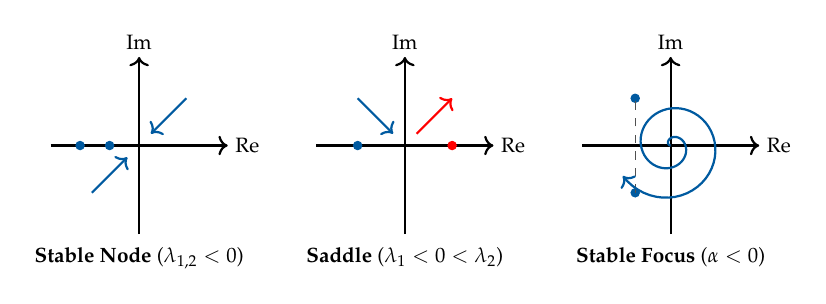
\begin{tikzpicture}[scale=0.75, every node/.style={scale=0.75}]
\begin{scope}[shift={(0,0)}]
\draw[->, thick] (-1.5,0) -- (1.5,0) node[right] {Re};
\draw[->, thick] (0,-1.5) -- (0,1.5) node[above] {Im};
\draw[themeblue, fill=themeblue] (-0.5,0) circle (2pt);
\draw[themeblue, fill=themeblue] (-1.0,0) circle (2pt);
\draw[->, themeblue, thick] (0.8,0.8) -- (0.2,0.2);
\draw[->, themeblue, thick] (-0.8,-0.8) -- (-0.2,-0.2);
\node[below] at (0,-1.6) {\textbf{Stable Node} ($\lambda_{1,2} < 0$)};
\end{scope}
\begin{scope}[shift={(4.5,0)}]
\draw[->, thick] (-1.5,0) -- (1.5,0) node[right] {Re};
\draw[->, thick] (0,-1.5) -- (0,1.5) node[above] {Im};
\draw[themeblue, fill=themeblue] (-0.8,0) circle (2pt);
\draw[red, fill=red] (0.8,0) circle (2pt);
\draw[->, themeblue, thick] (-0.8,0.8) -- (-0.2,0.2);
\draw[->, red, thick] (0.2,0.2) -- (0.8,0.8);
\node[below] at (0,-1.6) {\textbf{Saddle} ($\lambda_1 < 0 < \lambda_2$)};
\end{scope}
\begin{scope}[shift={(9,0)}]
\draw[->, thick] (-1.5,0) -- (1.5,0) node[right] {Re};
\draw[->, thick] (0,-1.5) -- (0,1.5) node[above] {Im};
\draw[themeblue, fill=themeblue] (-0.6,0.8) circle (2pt);
\draw[themeblue, fill=themeblue] (-0.6,-0.8) circle (2pt);
\draw[dashed, themegray] (-0.6,-0.8) -- (-0.6,0.8);
\draw[->, themeblue, thick, domain=0:12, variable=\t, samples=100] plot ({-0.08*\t*cos(\t r)}, {0.08*\t*sin(\t r)});
\node[below] at (0,-1.6) {\textbf{Stable Focus} ($\alpha < 0$)};
\end{scope}
\end{tikzpicture}
\end{center}

\cheatsheetsection{Laplace Transforms \& Applied Analysis}
The Laplace Transform maps time-domain differential equations into frequency-domain ($s$-domain) algebraic equations: $F(s) = \mathcal{L}\{f(t)\} = \int_{0}^{\infty} e^{-st}f(t)dt$.

\cheatsheetsubsection{Handling Initial Conditions}
Laplace transforms intrinsically embed the system's initial conditions, bypassing the need to solve for integration constants later.
\begin{itemize}[leftmargin=*, nosep]
    \item $\mathcal{L}\{y'(t)\} = sY(s) - y(0)$
    \item $\mathcal{L}\{y''(t)\} = s^2Y(s) - sy(0) - y'(0)$
    \item $\mathcal{L}\{y^{(n)}(t)\} = s^nY(s) - s^{n-1}y(0) - \dots - y^{(n-1)}(0)$
\end{itemize}

\newpage
\cheatsheetsubsection{Method of Partial Fractions}
Essential for performing the Inverse Laplace Transform $\mathcal{L}^{-1}$ on complex rational functions $F(s) = P(s)/Q(s)$.
\textbf{Step 1:} Fully factor the denominator $Q(s)$. \\
\textbf{Step 2:} Construct the algebraic template based on the factors:
\begin{itemize}[leftmargin=*, nosep]
    \item \textbf{Linear Distinct:} For $(s-a)$, use $\frac{A}{s-a}$
    \item \textbf{Repeated Linear:} For $(s-a)^k$, use $\frac{A_1}{s-a} + \frac{A_2}{(s-a)^2} + \dots + \frac{A_k}{(s-a)^k}$
    \item \textbf{Irreducible Quadratic:} For $(s^2+as+b)$, use $\frac{As+B}{s^2+as+b}$
\end{itemize}
\textbf{Step 3:} Solve for the unknown coefficients ($A, B, \dots$) using the Heaviside cover-up method or by equating polynomial coefficients. \\
\textbf{Step 4:} Apply the inverse transform $\mathcal{L}^{-1}$ to each resulting simple fraction using the table.

\cheatsheetsubsection{Special Functions in Linear Systems}
\begin{itemize}[leftmargin=*, nosep]
    \item \textbf{Gamma Function $\Gamma(x)$:} The analytic continuation of the factorial function to complex/real numbers, defined as $\int_0^\infty t^{x-1}e^{-t}dt$. Properties: $\Gamma(n+1) = n!$ and $\Gamma(1/2) = \sqrt{\pi}$. It is strictly necessary when computing the Laplace transform of fractional power functions like $t^{3/2}$.
    \item \textbf{Heaviside Step Function $u_c(t)$ or $u(t-c)$:} Evaluates to $0$ for $t < c$ and $1$ for $t \ge c$. It acts as a mathematical switch, heavily utilized to model piecewise operations, delayed excitations, and digital logic signals in control systems.
    \item \textbf{Dirac Delta Function $\delta(t-c)$:} A generalized function (distribution) representing an infinitely concentrated impulse at $t=c$. It has an infinite peak but finite integral $\int \delta(t-c)dt = 1$. Used to simulate instantaneous mechanical shocks, lightning strikes, or impulsive forces.
\end{itemize}

\newpage
\cheatsheetsection{Laplace Properties \& Operational Identities}
\vspace{0.2em}
\renewcommand{\arraystretch}{1.2}
\begin{tabularx}{\linewidth}{|p{0.35\linewidth}|X|}
\hline
\textbf{Theorem / Property} & \textbf{Mathematical Identity} \\ \hline
Linearity & $\mathcal{L}\{af(t) + bg(t)\} = aF(s) + bG(s)$ \\ \hline
First Shifting Theorem & $\mathcal{L}\{e^{at}f(t)\} = F(s-a)$ \\ \hline
Second Shifting Theorem & $\mathcal{L}\{u_c(t)f(t-c)\} = e^{-cs}F(s)$ \\ \hline
Integral Transform & $\mathcal{L}\{\int_0^t f(\tau)d\tau\} = \frac{F(s)}{s}$ \\ \hline
Multiplication by $t^n$ & $\mathcal{L}\{t^n f(t)\} = (-1)^n \frac{d^n}{ds^n}F(s)$ \\ \hline
Division by $t$ & $\mathcal{L}\{\frac{f(t)}{t}\} = \int_s^\infty F(u)du$ \\ \hline
Convolution Theorem & $\mathcal{L}\{(f * g)(t)\} = F(s)G(s)$ \\ \hline
Periodic Function ($T$) & $\mathcal{L}\{f(t)\} = \frac{1}{1-e^{-sT}} \int_0^T e^{-st}f(t)dt$ \\ \hline
\end{tabularx}

\cheatsheetsection{Common Pitfalls \& Errors in Laplace}
\begin{itemize}[leftmargin=*, nosep]
    \item \textbf{Linearity Violation in Multiplication:} Assuming $\mathcal{L}\{f(t)g(t)\} = F(s)G(s)$. This is false; multiplication in the time domain requires complex convolution in the $s$-domain.
    \item \textbf{Incorrect Time Shifting (Inverse):} Forgetting to shift the time argument of the function when returning from an exponential in the $s$-domain. $\mathcal{L}^{-1}\{e^{-cs}F(s)\} = u_c(t)f(t-c)$, not $u_c(t)f(t)$.
    \item \textbf{Incomplete Quadratic Numerator:} Setting up a partial fraction for an irreducible quadratic like $s^2+4$ using only $A$ in the numerator instead of $As+B$.
\end{itemize}

\clearpage 

\begingroup
\large
\renewcommand{\arraystretch}{1.4}

\cheatsheetsection{Table of Common Laplace Transforms}
\vspace{0.5em}

\begin{tabularx}{\linewidth}{|p{0.45\linewidth}|X|}
\hline
\textbf{Function $f(t) = \mathcal{L}^{-1}\{F(s)\}$} & \textbf{Transform $F(s) = \mathcal{L}\{f(t)\}$} \\ \hline
$1$ & $\frac{1}{s}$ \\ \hline
$t^n \quad (n = 1,2,3,\dots)$ & $\frac{n!}{s^{n+1}}$ \\ \hline
$t^p \quad (p > -1)$ & $\frac{\Gamma(p+1)}{s^{p+1}}$ \\ \hline
$\sqrt{t}$ & $\frac{\sqrt{\pi}}{2s^{3/2}}$ \\ \hline
$t^{n-1/2} \quad (n = 1,2,\dots)$ & $\frac{1 \cdot 3 \dots (2n-1)\sqrt{\pi}}{2^n s^{n+1/2}}$ \\ \hline
$e^{at}$ & $\frac{1}{s-a}$ \\ \hline
$t^n e^{at}$ & $\frac{n!}{(s-a)^{n+1}}$ \\ \hline
$\sin(at)$ & $\frac{a}{s^2+a^2}$ \\ \hline
$\cos(at)$ & $\frac{s}{s^2+a^2}$ \\ \hline
$\sinh(at)$ & $\frac{a}{s^2-a^2}$ \\ \hline
$\cosh(at)$ & $\frac{s}{s^2-a^2}$ \\ \hline
$t \sin(at)$ & $\frac{2as}{(s^2+a^2)^2}$ \\ \hline
$t \cos(at)$ & $\frac{s^2-a^2}{(s^2+a^2)^2}$ \\ \hline
$t \sinh(at)$ & $\frac{2as}{(s^2-a^2)^2}$ \\ \hline
$t \cosh(at)$ & $\frac{s^2+a^2}{(s^2-a^2)^2}$ \\ \hline
$e^{at}\sin(bt)$ & $\frac{b}{(s-a)^2+b^2}$ \\ \hline
$e^{at}\cos(bt)$ & $\frac{s-a}{(s-a)^2+b^2}$ \\ \hline
$e^{at}\sinh(bt)$ & $\frac{b}{(s-a)^2-b^2}$ \\ \hline
$e^{at}\cosh(bt)$ & $\frac{s-a}{(s-a)^2-b^2}$ \\ \hline
\end{tabularx}

\newpage

\cheatsheetsection{Table of Common Laplace Transforms}
\vspace{0.5em}

\begin{tabularx}{\linewidth}{|p{0.45\linewidth}|X|}
\hline
\textbf{Function $f(t) = \mathcal{L}^{-1}\{F(s)\}$} & \textbf{Transform $F(s) = \mathcal{L}\{f(t)\}$} \\ \hline
$\sin(at) - at \cos(at)$ & $\frac{2a^3}{(s^2+a^2)^2}$ \\ \hline
$\sin(at) + at \cos(at)$ & $\frac{2as^2}{(s^2+a^2)^2}$ \\ \hline
$\cos(at) - at \sin(at)$ & $\frac{s(s^2-a^2)}{(s^2+a^2)^2}$ \\ \hline
$\cos(at) + at \sin(at)$ & $\frac{s(s^2+3a^2)}{(s^2+a^2)^2}$ \\ \hline
$u_c(t)$ or $u(t-c)$ & $\frac{e^{-cs}}{s}$ \\ \hline
$\delta(t-c)$ & $e^{-cs}$ \\ \hline
$1 - \cos(at)$ & $\frac{a^2}{s(s^2+a^2)}$ \\ \hline
$at - \sin(at)$ & $\frac{a^3}{s^2(s^2+a^2)}$ \\ \hline
$\frac{1}{a-b}(e^{at} - e^{bt})$ & $\frac{1}{(s-a)(s-b)}$ \\ \hline
$\frac{1}{a-b}(a e^{at} - b e^{bt})$ & $\frac{s}{(s-a)(s-b)}$ \\ \hline
$\frac{1}{t}\sin(at)$ & $\arctan\left(\frac{a}{s}\right)$ \\ \hline
$\frac{1}{t}(1 - \cos(at))$ & $\frac{1}{2}\ln\left(\frac{s^2+a^2}{s^2}\right)$ \\ \hline
$\frac{1}{t}(1 - e^{-at})$ & $\ln\left(\frac{s+a}{s}\right)$ \\ \hline
$J_0(at)$ (Bessel function) & $\frac{1}{\sqrt{s^2+a^2}}$ \\ \hline
$J_0(2\sqrt{kt})$ & $\frac{1}{s}e^{-k/s}$ \\ \hline
$\frac{1}{\sqrt{\pi t}}e^{-a^2/4t}$ & $\frac{1}{\sqrt{s}}e^{-a\sqrt{s}}$ \\ \hline
$\frac{a}{2\sqrt{\pi t^3}}e^{-a^2/4t}$ & $e^{-a\sqrt{s}}$ \\ \hline
$e^{at} - at - 1$ & $\frac{a^2}{s^2(s-a)}$ \\ \hline
$f(t) * g(t)$ (Convolution) & $F(s)G(s)$ \\ \hline
\end{tabularx}
\endgroup

\clearpage
\onecolumn

\cheatsheetsection{ODE Solution Strategy Decision Tree}
\vspace{1em}

\begin{center}
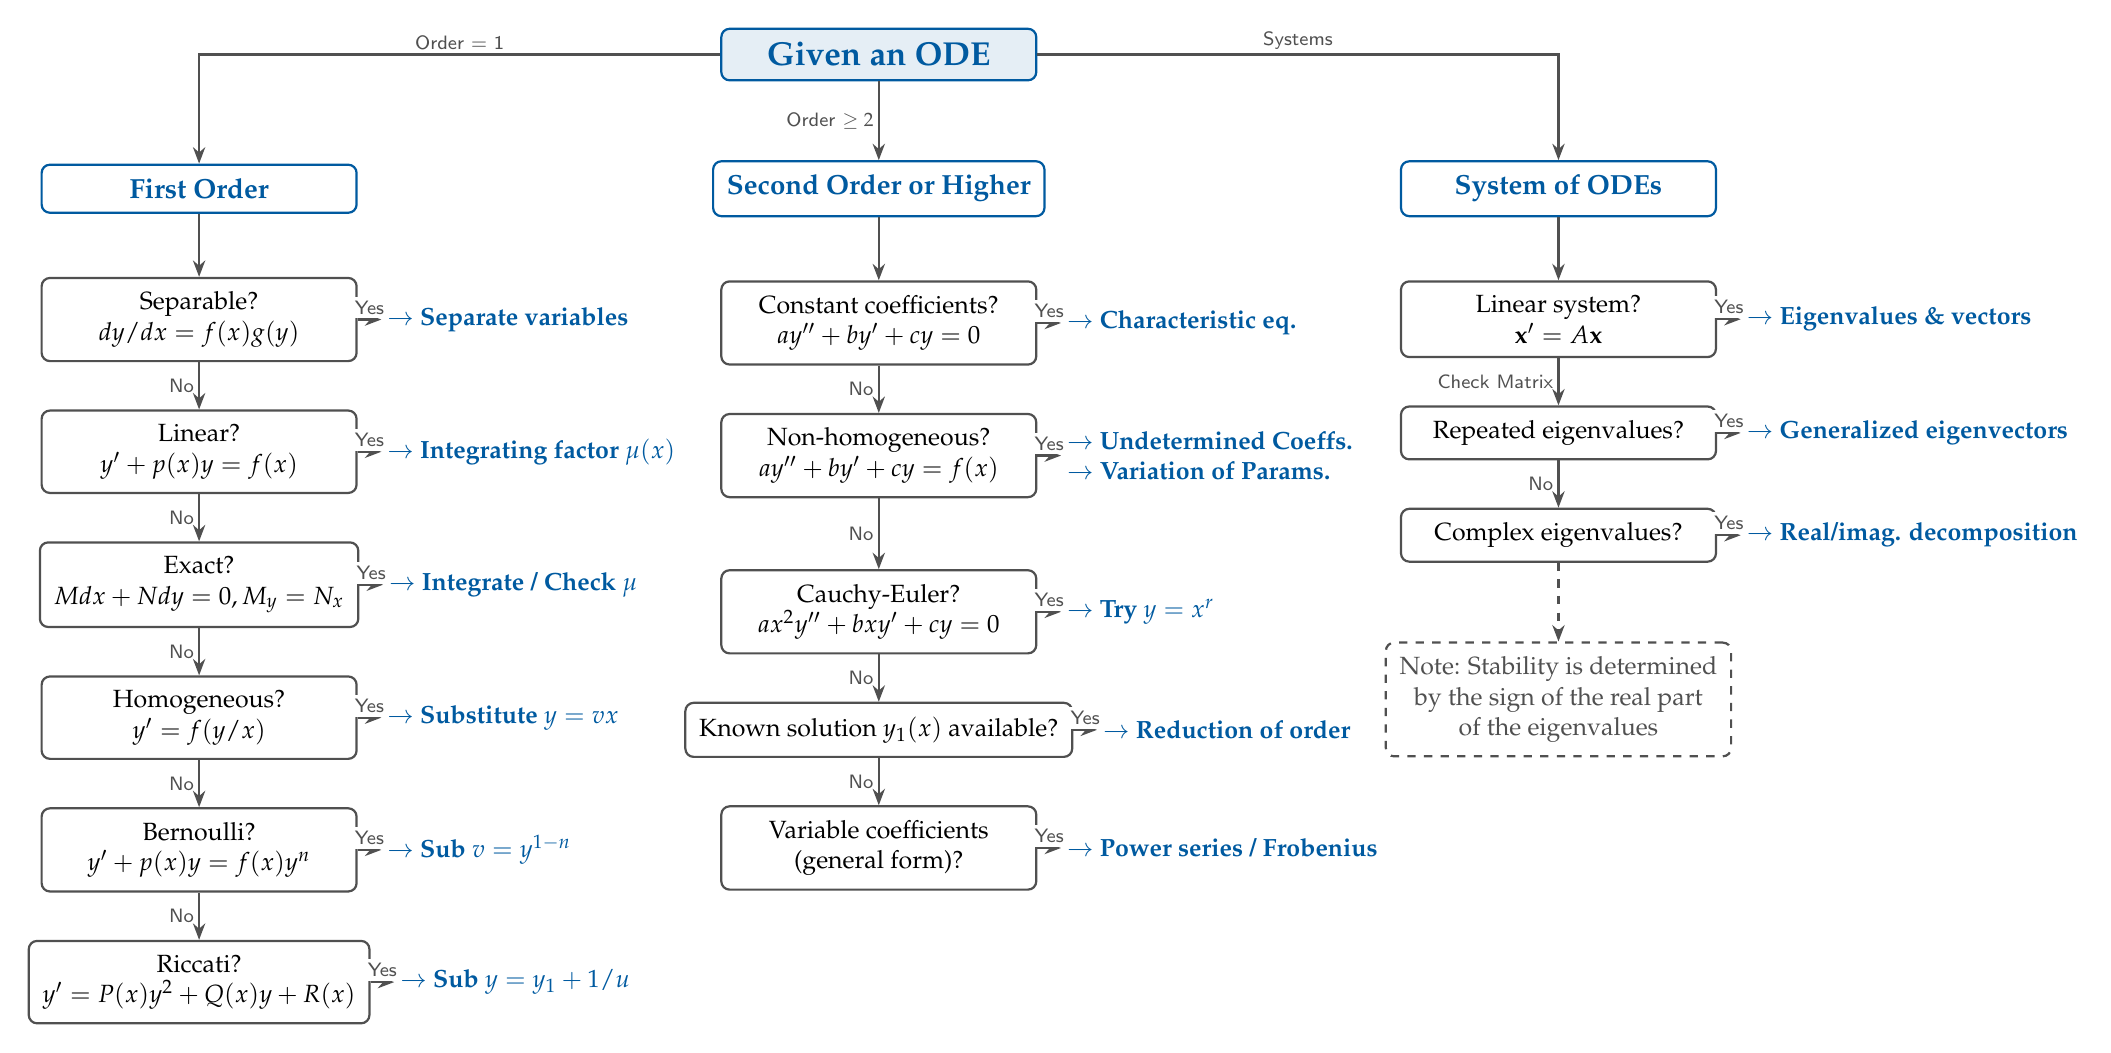
\begin{tikzpicture}[
    node distance=0.6cm and 0.8cm,
    base/.style={rectangle, rounded corners=3pt, draw=themegray, thick, align=center, font=\small, inner sep=5pt},
    root/.style={base, draw=themeblue, fill=themeblue!10, text=themeblue, font=\large\bfseries, minimum width=4cm},
    category/.style={base, draw=themeblue, fill=white, text=themeblue, font=\normalsize\bfseries, minimum width=4cm},
    decision/.style={base, fill=white, minimum width=4cm, text=black},
    method/.style={rectangle, align=left, text=themeblue, font=\small\bfseries, inner sep=2pt},
    line/.style={draw=themegray, thick, -{Stealth[scale=0.9]}},
    label/.style={font=\scriptsize\sffamily, text=themegray, fill=white, inner sep=1.5pt}
]

\node[root] (start) {Given an ODE};

\node[category, below=1cm of start] (second) {Second Order or Higher};
\node[category, left=4.5cm of second] (first) {First Order};
\node[category, right=4.5cm of second] (system) {System of ODEs};

\draw[line] (start) -| node[label, near start, above] {Order = 1} (first);
\draw[line] (start) -- node[label, fill=none, left] {Order $\ge 2$} (second);
\draw[line] (start) -| node[label, near start, above] {Systems} (system);

\node[decision, below=0.8cm of first] (sep) {Separable?\\$dy/dx = f(x)g(y)$};
\node[method, right=0.3cm of sep] (m_sep) {$\rightarrow$ Separate variables};

\node[decision, below=0.6cm of sep] (lin) {Linear?\\$y' + p(x)y = f(x)$};
\node[method, right=0.3cm of lin] (m_lin) {$\rightarrow$ Integrating factor $\mu(x)$};

\node[decision, below=0.6cm of lin] (exact) {Exact?\\$M dx + N dy = 0, M_y=N_x$};
\node[method, right=0.3cm of exact] (m_exact) {$\rightarrow$ Integrate / Check $\mu$};

\node[decision, below=0.6cm of exact] (homo) {Homogeneous?\\$y' = f(y/x)$};
\node[method, right=0.3cm of homo] (m_homo) {$\rightarrow$ Substitute $y = vx$};

\node[decision, below=0.6cm of homo] (ber) {Bernoulli?\\$y' + p(x)y = f(x)y^n$};
\node[method, right=0.3cm of ber] (m_ber) {$\rightarrow$ Sub $v = y^{1-n}$};

\node[decision, below=0.6cm of ber] (ric) {Riccati?\\$y' = P(x)y^2 + Q(x)y + R(x)$};
\node[method, right=0.3cm of ric] (m_ric) {$\rightarrow$ Sub $y = y_1 + 1/u$};

\draw[line] (first) -- (sep);
\draw[line] (sep) -- node[label, above] {Yes} (m_sep);
\draw[line] (sep) -- node[label, fill=none, left] {No} (lin);
\draw[line] (lin) -- node[label, above] {Yes} (m_lin);
\draw[line] (lin) -- node[label, fill=none, left] {No} (exact);
\draw[line] (exact) -- node[label, above] {Yes} (m_exact);
\draw[line] (exact) -- node[label, fill=none, left] {No} (homo);
\draw[line] (homo) -- node[label, above] {Yes} (m_homo);
\draw[line] (homo) -- node[label, fill=none, left] {No} (ber);
\draw[line] (ber) -- node[label, above] {Yes} (m_ber);
\draw[line] (ber) -- node[label, fill=none, left] {No} (ric);
\draw[line] (ric) -- node[label, above] {Yes} (m_ric);

\node[decision, below=0.8cm of second] (const) {Constant coefficients?\\$ay''+by'+cy=0$};
\node[method, right=0.3cm of const] (m_const) {$\rightarrow$ Characteristic eq.};

\node[decision, below=0.6cm of const] (nonhomo) {Non-homogeneous?\\$ay''+by'+cy=f(x)$};
\node[method, right=0.3cm of nonhomo, align=left] (m_nonhomo) {$\rightarrow$ Undetermined Coeffs.\\$\rightarrow$ Variation of Params.};

\node[decision, below=0.9cm of nonhomo] (euler) {Cauchy-Euler?\\$ax^2y''+bxy'+cy=0$};
\node[method, right=0.3cm of euler] (m_euler) {$\rightarrow$ Try $y = x^r$};

\node[decision, below=0.6cm of euler] (known) {Known solution $y_1(x)$ available?};
\node[method, right=0.3cm of known] (m_known) {$\rightarrow$ Reduction of order};

\node[decision, below=0.6cm of known] (var) {Variable coefficients\\(general form)?};
\node[method, right=0.3cm of var] (m_var) {$\rightarrow$ Power series / Frobenius};

\draw[line] (second) -- (const);
\draw[line] (const) -- node[label, above] {Yes} (m_const);
\draw[line] (const) -- node[label, fill=none, left] {No} (nonhomo);
\draw[line] (nonhomo) -- node[label, above] {Yes} (m_nonhomo);
\draw[line] (nonhomo) -- node[label, fill=none, left] {No} (euler);
\draw[line] (euler) -- node[label, above] {Yes} (m_euler);
\draw[line] (euler) -- node[label, fill=none, left] {No} (known);
\draw[line] (known) -- node[label, above] {Yes} (m_known);
\draw[line] (known) -- node[label, fill=none, left] {No} (var);
\draw[line] (var) -- node[label, above] {Yes} (m_var);


\node[decision, below=0.8cm of system] (linsys) {Linear system?\\$\mathbf{x}' = A\mathbf{x}$};
\node[method, right=0.3cm of linsys] (m_linsys) {$\rightarrow$ Eigenvalues \& vectors};

\node[decision, below=0.6cm of linsys] (rep) {Repeated eigenvalues?};
\node[method, right=0.3cm of rep] (m_rep) {$\rightarrow$ Generalized eigenvectors};

\node[decision, below=0.6cm of rep] (comp) {Complex eigenvalues?};
\node[method, right=0.3cm of comp] (m_comp) {$\rightarrow$ Real/imag. decomposition};

\node[base, draw=themegray, dashed, below=1cm of comp, text=themegray] (stab) {Note: Stability is determined\\by the sign of the real part\\of the eigenvalues};

\draw[line] (system) -- (linsys);
\draw[line] (linsys) -- node[label, above] {Yes} (m_linsys);
\draw[line] (linsys) -- node[label, fill=none, left] {Check Matrix} (rep);
\draw[line] (rep) -- node[label, above] {Yes} (m_rep);
\draw[line] (rep) -- node[label, fill=none, left] {No} (comp);
\draw[line] (comp) -- node[label, above] {Yes} (m_comp);

\draw[line, dashed, draw=themegray] (comp) -- (stab);

\end{tikzpicture}
\end{center}

\end{document}